\section{Proofs}
\label{sec:proofs}

In Section~\ref{sec:analysis:definitions} we introduce some formalisms.
In Section~\ref{subsec:Generic-algorithm-proof} we prove that
the unoptimised algorithm is strongly linearisable with respect to
the relaxed specification $SeqSketch^r$ with $r=Nb$. Finally,
in Section~\ref{subsec:Optimised-algorithm-proof} we show that
the the optimised algorithm is strongly linearisable with respect to
the relaxed specification $SeqSketch^r$ with $r=2Nb$.

\subsection{Definitions}
\label{sec:analysis:definitions}
Note that the only methods invoked by $ParSketch$ on $globalS$ are snapshot and merge, and since merge is
only invoked by $t_0$, the only concurrency is between a snapshot and another operation (snapshot or merge).
Recall that we required such executions of a composable sketch to be strongly linearisable. By slight abuse
of terminology, we refer to these operations as atomic steps, for example, we refer to the linearisation
point of $globalS$.merge simply as ``$globalS$.merge step''.

Likewise, as $localS_i$ is only accessed sequentially by a
single thread, either $t_i$ or $t_0$ (using $prop_i$ to synchronise),
we refer to the method calls shouldAdd and update as atomic steps.

Because we prove only safety properties, we restrict out attention to finite executions.
For analysis purposes we use abstract counters:
\begin{itemize}
    \item An array $sig\_ctr[N]$, that counts the number of times each thread $t_i$ signals to the propagator (line~\ref{l:signal}).
    \item An array $merge\_ctr[N]$ counting the number of times $t_0$ executes a merge with thread $t_i$'s local sketch (line~\ref{l:merge}).
\end{itemize}

Recall that in Section~\ref{sec:background}, we said that a sketch \emph{summarises} a
stream or a sequential history if its state is the state of a sketch that has processed
the stream or history. We now overload the term ``summarises'' to apply also to threads.
\begin{definition}[Thread summary]
    Consider a time $t$ in an execution $\sigma$ of Algorithm~\ref{alg:generic-concurrent}. If at time $t$ either $prop_i \neq 0$
    or $sig\_ctr[i]>merge\_ctr[i]$, then we say that update thread $t_i$ \emph{summarises} the history
    summarised by $localS_i$ at time $t$. Otherwise, thread $t_i$ summarises the empty history at time $t$.
    The propagator thread $t_0$ summarises the same history as $globalS$ at any time during an execution $\sigma$.
\label{def:thread-summary}
\end{definition}

As we want to analyse each thread's steps in an execution, we first define the projection from
execution $\sigma$ onto a thread $t_i$.
\begin{definition}[Projection]
    Given a finite execution $\sigma$ and a thread $t_i$, $\sigma\Bigr|_{t_i}$ is the subsequence of
    $\sigma$ consisting of steps taken by $t_i$.
\end{definition}

We want to prove that each thread's summary corresponds to the sequence of updates
processed by that thread since the last propagation, taking
into account only those that alter local state variables. These are updates for which \emph{shouldAdd} returns
true.
\begin{definition}[Unprop updates]
    Given a finite execution $\sigma$, we denote by suff$_i(\sigma)$ the suffix of $\sigma \Bigr|_{t_i}$ starting 
    at the last $globalS$.merge($localS_i$) event, or the beginning of $\sigma$ if no such event exists. 
    The unprop suffix up\_suff$_i(\sigma)$ of update thread $i$ is 
    the subsequence of $\mathcal{H} ($suff$_i(\sigma))$ consisting of $update(a)$ executions in suff$_i(\sigma)$ for which
    shouldAdd$(hint_i, arg)$ returns true in line \ref{l:shouldAdd}.
    \label{def:unpropogated-suffix}
\end{definition}

We define the relation between a sequential history $H$ and a stream $A$.
\begin{definition}
    Given a finite sequential history $H$, ${\mathcal{S}}(H)$ is the stream $a_1,\dots,a_n$ such that $a_k$
    is the argument of the $k$th update in $H$.
\end{definition}

Finally, we define the notion of \emph{happens before} in a sequential history $H$.
\begin{definition}
    Given a finite sequential history $H$ and two method invocations $M_1,M_2$ in $H$, we denote $M_1 \prec_H M_2$
    if $M_1$ precedes $M_2$ in $H$.
\end{definition}

\subsection{Unoptimised algorithm proof} 
\label{subsec:Generic-algorithm-proof}

Our strong linearisability proof uses two mappings, $f$ and $l$, from 
executions to sequential histories defined as follows.
For an execution $\sigma$ of $ParSketch$, we define a mapping $f$ 
by ordering operations according to \emph{visibility points} defined as follows: 
\begin{itemize}
\item
For a query, the visibility point is the snapshot operation it executes.
\item 
For an update$_i$($a$) where shouldAdd($prop_i$, $a$) returns false at time $t$, its visibility point is $t$.
\item
Otherwise, for an update$_i$($a$), let $t$ be the first time after its invocation in $\sigma$
when thread $i$ changes $prop_i$ to 0 (line~\ref{l:signal}).
Its visibility point is the (linearisation point of the) first merge that occurs with $localS_i$ after time t.
If there is no such time, then update$_i$($a$) does not have a visibility point, i.e., is not included in $f(\sigma)$
\end{itemize}
Note that in the latter case,
the visibility point may occur after the update returns, and so $f$ does not 
necessarily preserve real-time order. 
 
We also define a mapping $l$ by ordering operations according to
\emph{linearisation points} define as follows:
\begin{itemize}
    \item
    An updates' linearisation point is its invocation
    \item
    A query's linearisation point is its visibility point.
\end{itemize}
By definition, $l(\sigma)$ is prefix-preserving.

We show that for every execution $\sigma$ of $ParSketch$,
(1) $f(\sigma) \in SeqSketch$, and 
(2) $f(\sigma)$ is an $r$-relaxation of $l(\sigma)$ for $r=N b$.  
Together, this implies that $l(\sigma) \in SeqSketch^r$, as needed.

We first show that $Prop_i \neq 0$ if $t_i$'s program counter is not on lines \ref{l:signal} or \ref{l:wait}.
\begin{invariant}
    At any time during a finite execution $\sigma$ of $ParSketch$ for every $i=1,\dots,N$, if $t_i$'s program
    counter isn't on lines \ref{l:signal} or \ref{l:wait}, then $prop_i \neq 0$.
    \label{inv:prop-neq-0}
\end{invariant}
\begin{proof}
    The proof is derived immediately from the algorithm: $prop_i$ is initialised to 1 and gets
    the value of 0 on line \ref{l:signal}, and then waits on line \ref{l:wait} until $prop_i \neq 0$.
    After continuing passed line \ref{l:wait}, $prop_i \neq 0$ again.
\end{proof}

We also observe the following:
\begin{observation}
    Given a finite execution $\sigma$ of $ParSketch$, for every $i=1,\dots,N$, every execution
    of $globalS.merge(localS_i)$ in $\sigma$ (line~\ref{l:merge}) is preceded by an execution of $prop_i \leftarrow 0$
    (line~\ref{l:signal}).
\end{observation}

We observe the following relationship between $t_i$'s program counter and $sig\_ctr[i]$ and \linebreak
$merge\_ctr[i]$:
\begin{observation}
    At all times during a finite execution $\sigma$ of $ParSketch$, for every
    $i=1,\dots,N$, $merge\_ctr[i] \leq sig\_ctr[i] \leq merge\_ctr[i] + 1$.
    Moreover, if $t_i$'s program counter isn't on lines \ref{l:signal} or \ref{l:wait}, then $sig\_ctr[i]=merge\_ctr[i]$.
    \label{obs:counter_relationship}
\end{observation}

We show that at every point in an execution, update thread $t_i$ summarises up\_suff$_i(\sigma)$. 
In essence, this means that we have not ``forgotten" any updates.
\begin{invariant}
    At all times during a finite execution $\sigma$ of $ParSketch$, for every $i=1,\dots,N$, $t_i$ summarises up\_suff$_i(\sigma)$.
    \label{inv:update-thread-summary}
\end{invariant}
\begin{proof}
    The proof is by induction on the length of $\sigma$. The base is immediate.
    Next we consider a step in $\sigma$ that can alter the invariant. We assume the invariant is correct
    for $\sigma'$, and prove correctness for $\sigma=\sigma',step$. We consider ony steps that
    can alter the invariant, meaning the step can 
    either lead to a change in up\_suff$_i(\sigma)$, or a change in the history summarised by $t_i$. This
    means we need consider only 4 cases:
    \begin{itemize}

        \item A step $localS_i.update(arg)$ (line~\ref{l:update}) by thread $t_i$.

        In this case, up\_suff$_i(\sigma)=$up\_suff$_i(\sigma'),update(arg)$.
        By the inductive hypothesis, before the step $localS_i$ summarises up\_suff$_i(\sigma')$,
        and so after the update, $localS_i$ summarises $\text{up\_suff}_i(\sigma'),$ \linebreak $update(arg)=\text{up\_suff}_i(\sigma)$.
        From Invariant~\ref{inv:prop-neq-0} $prop_i \neq 0$, therefore, by Definition \ref{def:thread-summary}, $t_i$ summarises
        the same history as $localS_i$,
        i.e., up\_suff$_i(\sigma)$, preserving the invariant.

        \item A step $prop_i \leftarrow 0$ (line~\ref{l:signal}) by thread $t_i$.
        
        By the inductive hypothesis, before the step $localS_i$ and $t_i$ summarise the same
        history up\_suff$_i(\sigma')$.
        As no update occurs, up\_suff$_i(\sigma')$$=$up\_suff$_i(\sigma)$. The step
        doesn't alter $localS_i$, so after the step, $localS_i$ still summarises
        up\_suff$_i(\sigma)$. On this step the counter $sig\_ctr[i]$ is increased but $merge\_ctr[i]$
        is not, so $sig\_ctr[i]>merge\_ctr[i]$.
        Therefore, by Definition \ref{def:thread-summary}, $t_i$ summarises the same history as $localS_i$,
        namely up\_suff$_i(\sigma)$, preserving the invariant.

        \item A step $globalS.merge(localS_i)$ (line~\ref{l:merge}) by thread $t_0$.
        
        By Definition~\ref{def:unpropogated-suffix}, after this step up\_suff$_i(\sigma)$ is empty. As
        this step is a $merge$, $merge\_ctr[i]$ is increased by one, so $sig\_ctr[i]=merge\_ctr[i]$ by
        Observation~\ref{obs:counter_relationship}.
        Therefore, by Definition \ref{def:thread-summary}, $t_i$
        summarises the empty history, preserving the invariant.

        \item A step $prop_i \leftarrow globalS.calcHint()$ (line~\ref{l:calcHint}) by thread $t_0$
        
        Before executing the step, $t_0$ executed line~\ref{l:emptyAux}. Thread $t_i$ is waiting
        for $prop_i \neq 0$ on line~\ref{l:wait}, therefore has not updated $localS_i$.
        Therefore, $localS_i$ summarises the empty history.
        As a merge with thread $i$ was executed and no updates have been invoked, up\_suff$_i(\sigma)$
        is the empty history.
        The function $calcHint$ cannot return $0$, therefore after the step $prop_i \neq 0$.
        By Definition \ref{def:thread-summary}, $t_i$ summarises the same history as $localS_i$, i.e., the empty history.
        Therefore, $t_i$ summarises up\_suff$_i(\sigma)$, preserving the invariant.
    \end{itemize}
\end{proof}

Next, we prove that $t_0$ summarises $f(\sigma)$.
\begin{invariant}[History of propagator thread]
    Given a finite execution $\sigma$ of $ParSketch$, $t_0$ summarises $f(\sigma)$.
    \label{inv:G-partial-summary}
\end{invariant}
\begin{proof}
    The proof is by induction on the length of $\sigma$. The base is immediate.
    We assume the invariant is correct for $\sigma'$, and prove correctness for $\sigma=\sigma',step$.
    There are two steps that can alter the invariant.
    \begin{itemize}
        \item A step $globalS.merge(localS_i)$ (line~\ref{l:merge}) by thread $t_0$.
        
        By the inductive hypothesis, before the step, $t_0$ summarises $f(\sigma')$. And by
        Invariant~\ref{inv:update-thread-summary}, before the update, $t_i$ summarises
        up\_suff$_i(\sigma')$, and bu Invariant~\ref{inv:prop-neq-0} $localS_i$ summarises the same history.
        Let $A={\mathcal{S}}(f(\sigma))$, and $B={\mathcal{S}}($up\_suff$_i(\sigma')$$)$.
        After the merge $globalS$ summarises $A||B$. Therefore,
        $t_0$ summarises $f(\sigma)$ preserving the invariant.

        \item A step shouldAdd($prop_i$, $a$) (line~\ref{l:shouldAdd}) by thread $t_i$, returning false.     
        
        Let $H$ be that last hint returned to $t_i$, and let $\sigma''$ be the prefix of $\sigma$ up to this point.
        By the induction hypothesis, at that point $globalS$ summarised $f(\sigma'')$.
        Let $A=\mathcal{S}$$(f(\sigma''))$, and let $B=\mathcal{S}$$(f(\sigma'))$,
        and let $B_1$ be such that $B=A||B_1$. By the induction hypothesis,
        before the step, $globalS$ summarises $B=A||B_1$.
        By the assumption of \emph{shouldAdd}, if shouldAdd($H$, $arg$) returns false, then if
        a sketch summarises $B=A||B_1||B_2$, then it also summarises $B=A||B_1||a||B_2$. Let
        $B_2=\emptyset$, then $globalS$ summarises $B=A||B_1||B_2$, therefore also summarises 
        $A||B_1||a||B_2=A||B_1||a$. Therefore, after the step, $globalS$ summarises $f(\sigma)$
        preserving the invariant.
    \end{itemize}
\end{proof}

To finish the proof that $f(\sigma) \in SeqSketch$, we prove that a query invoked at the end of $\sigma$
returns a value equal to the value returned by a sequential sketch after processing $A={\mathcal{S}}(f(\sigma))$.
\begin{lemma}[Query Correctness]
    Given a finite execution $\sigma$ of $ParSketch$, let $Q$ be a query that returns
    in $\sigma$, and let $v$ be $Q$'s visibility point. Let $\sigma'$ be the prefix
    of $\sigma$ until point $v$, and let $A={\mathcal{S}}(f(\sigma'))$. $Q$ returns a value
    that is equal to the value returned by a sequential sketch after processing $A$.
    \label{lemma:query-correctness}
\end{lemma}
\begin{proof}
    Let $\sigma$ be an execution of $ParSketch$, and let $Q$ be a query that returns in $\sigma$.
    Let $\sigma'$ and $A$ be as defined in the lemma. By Invariant \ref{inv:G-partial-summary}, 
    $t_0$ summarises $f(\sigma')$ at point $v$, therefore \emph{globalS} 
    summarises $f(\sigma')$ at the same point, therefore \emph{globalS} summarises 
    stream $A$ at point $v$. The visibility point for the query, at point $v$,
    is $globalS.$snapshot$()$. By the requirement from $S$.snapshot(), for all $arg$ 
    $globalS.query(arg)=localCopy.query(arg)$. Because $globalS$ summarises
    stream $A$, $localCopy.query(arg)$ returns a value equal to the value
    returned by the sequential sketch $globalS$ after processing $A$.
\end{proof}

As we have proven that each query in $f(\sigma)$ returns a value that estimates all
the updates that happen before its invocation, we have proven the following:
\begin{lemma}
    Given a finite execution $\sigma$ of $ParSketch$, $f(\sigma) \in SeqSketch$.
    \label{lemma:f-in-seqsketch}
\end{lemma}

To complete the proof, we prove that $f(\sigma)$ is an $r$-relaxation of $l(\sigma)$, for $r=Nb$.
We begin by proving orders between queries and other method calls.
\begin{lemma}
    Given a finite execution $\sigma$ of $ParSketch$, and given an operation $O$(query or update) in $l(\sigma)$,
    for every $Q$ in $l(\sigma)$ such that $Q \prec_{l(\sigma)} O$,
    then $Q \prec_{f(\sigma)} O$.
    \label{lemma:QueryOrders}
\end{lemma}
\begin{proof}
    If $O$ is a query,
    then proof is immediate from the definitions of $l$ and $f$.
    If $O$ is an update, then, by the definition of $f$, an updates visibility point
    is at the earliest its linearisation point.
    As $Q$'s visibility point and linearisation point are equal, it follows
    that if  $Q \prec_{l(\sigma)} O$ then $Q \prec_{f(\sigma)} O$.
\end{proof}

We next prove an upper bound on the number of updates in up\_suff$_i(\sigma)$. We denote the
number of updates in history $H$ as $\abs{H}$.
\begin{lemma}
    Given a finite execution $\sigma$ of $ParSketch$, $\abs{\text{up\_suff}_i(\sigma)} \leq b$.
    \label{lemma:update-thread-summary-bound}
\end{lemma}
\begin{proof}
    As $counter_i$ is incremented before an update which is included in $\text{up\_suff}_i(\sigma)$,
    it follows that $\abs{\text{up\_suff}_i(\sigma)} \leq counter_i$. When $counter_i = b$, $t_i$
    signals for a propagation (line~\ref{l:signal}) and then waits until $prop_i \neq 0$ (line~\ref{l:wait}).
    When $t_i$ finishes waiting, then it zeros the counter (line~\ref{l:zeroCounter}) before ingesting
    more updates, therefore, $count_i \leq b$. Therefore, it follows that $\abs{\text{up\_suff}_i(\sigma)} \leq b$.
\end{proof}

As $f(\sigma)$ contains all updates with visibility points, we can now prove the following.
\begin{lemma}
    Given a finite execution $\sigma$ of $ParSketch$, $\abs{f(\sigma)} \geq \abs{l(\sigma)} - N$$b$.
    \label{lemma:f-bound}
\end{lemma}
\begin{proof}
    From Lemma~\ref{lemma:update-thread-summary-bound}, $\abs{\text{up\_suff}_i(\sigma)} \leq b$.
    The only updates without a visibility point are updates that are in up\_suff$_i(\sigma)$ for some $i$.
    Therefore $f(\sigma)$ contains all updates but any update in a history up\_suff$_i(\sigma)$ for some $i$.
    There are $N$ update threads, therefore $\abs{f(\sigma)} = \abs{l(\sigma)} - $$\sum_{i=1}^{N} \abs{\text{up\_suff}_i(\sigma)}$
    so $\abs{f(\sigma)} \geq \abs{l(\sigma)} - N $$b$.
\end{proof}

We will now prove that given an execution $\sigma$ of $ParSketch$, every invocation in $f(\sigma)$
is preceded by all but at most $r$ of the invocations in $l(\sigma)$.
\begin{lemma}
    Given a finite execution $\sigma$ of $ParSketch$, $f(\sigma)$ is a r-relaxation of $l(\sigma)$.
    \label{lemma:f-relaxing-l}
\end{lemma}
\begin{proof}
    Let $\sigma$ be a finite execution of $ParSketch$, and consider an operation $O$ in $f(\sigma)$
    such that $O$ is also in $l(\sigma)$. Let $Ops = \Set{O'}{(O' \prec_{l(\sigma)} O) \wedge (O' \nprec_{f(\sigma)} O)}$.
    We show that $\abs{Ops} \leq r$.
    By Lemma~\ref{lemma:QueryOrders}, for every query $Q$ in $l(\sigma)$ such that $Q \prec_{l(\sigma)} O$,
    then $Q \prec_{f(\sigma)} O$, meaning $Q \notin Ops$.
    Let $\sigma^{pre}$ be a prefix and $\sigma^{post}$ a suffix of $\sigma$ such that
    $l(\sigma)=l(\sigma^{pre}),O,l(\sigma^{post})$. From Lemma~\ref{lemma:f-bound}, $\abs{f(\sigma^{pre})} \geq \abs{l(\sigma^{pre})} - r$.
    As $\abs{f(\sigma^{pre})}$ is the number of updates in $f(\sigma^{pre})$, and $\abs{l(\sigma^{pre})}$ is the number of updates
    in $l(\sigma^{pre})$, $f(\sigma^{pre})$ contains all but at most $r$ updates in $l(\sigma^{pre})$. As $l(\sigma^{pre})$
    contains all the updates that precede $O$. Meaning $Ops$ is all the updates in $l(\sigma^{pre})$ and not in
    $f(\sigma^{pre})$. Therefore, $\abs{Ops} = \abs{l(\sigma^{pre})} - \abs{f(\sigma^{pre})} \leq r$.
    Therefore, by Definition~\ref{def:r-relaxtion}, $f(\sigma)$ is an $r$-relaxation of $l(\sigma)$.
\end{proof}

Putting together Lemma~\ref{lemma:f-in-seqsketch} and Lemma~\ref{lemma:f-relaxing-l}, we have shown that
given a finite execution $\sigma$ of $ParSketch$, $f(\sigma) \in SeqSketch$ and $f(\sigma)$ is an $r$-relaxation
of $l(\sigma)$. We have proven Lemma~\ref{lemma:genereic-strong}.

\subsection{Optimised algorithm proof}
\label{subsec:Optimised-algorithm-proof}
We prove the correctness of the optimised algorithm by simulating the optimised version of 
Algorithm~\ref{alg:generic-concurrent} with the unoptimised version.
We denote the optimised version of Algorithm~\ref{alg:generic-concurrent} as 
\emph{OptParSketch}. We show a \emph{simulation relation}~\cite{lynch1996distributed},
thus proving that $OptParSketch$ is strongly linearisable with regards to $SeqSketch^{2Nb}$.

Consider an arbitrary worker thread $t_i$ for the optimised algorithm,
and simulate this thread using two worker threads $t_i^0,t_i^1$ of Algorithm~\ref{alg:generic-concurrent}.
To simulate $N$ worker threads, you need $2N$ threads, and they are mapped the same way.

The idea behind the simulation is that there is a delay in when the \emph{hint} returned to the worker thread
is used for pre processing, so we can simulate each thread by two thread. For example in Figure~\ref{fig:optimisedSimulation},
each block $A_i$ is a stream such that $b$ updates pass the test of \emph{shouldAdd} (except maybe $A_n$).
The stream processed by $t_i$ is $A=A_1||A_2||\dots||A_n$ and we assume $n$ is even.
Each $A_i$ is evaluated against the \emph{hint} written above it. The thread $t_i^0$ simulates processing
$A_1||A_3||\dots ||A_{n-1}$, and thread $t_i^1$ simulates processing $A_2||A_4||\dots||A_n$.

\begin{figure}[H]
    \centering
    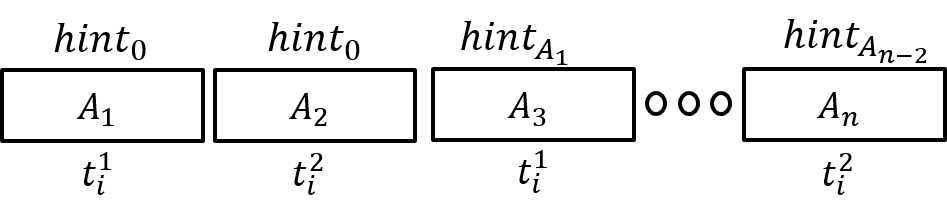
\includegraphics[width=5in]{images/optimisedSimulation.png}
    \caption{Simulation of processing $A=A_1||A_2||\dots||A_n$.}
    \label{fig:optimisedSimulation}
\end{figure}

The simulation uses abstract variables oldHint$_i^1$, and oldHint$_i^1$, both initialised to 1.
These variables are updated with the flipping of $cur_i$ (line~\ref{opt:l:swap-local-aux}), such that:
\begin{itemize}
    \item oldHint$_i^1$ is updated with the current (pre-flip) value of $hint_i$
    \item oldHint$_i^2$ is updated with the current (pre-flip) value of $oldHint_i^0$
\end{itemize}

%The simulation uses an abstract variable $oldHint_i^0$ initialised to 1. This variable is updated
%with the flipping of $cur_i$ (line~\ref{opt:l:swap-local-aux}) with the current value of $hint_i$.

In addition, the simulation uses an abstract variable \emph{auxCount$_i$} initialised to 0. This variable is set to
$b$ before the first execution of line~\ref{opt:l:swap-local-aux}, and is never changed after that. 

Finally, the simulation uses two abstract variables $PC_i^0$ and $PC_i^1$ to be
program counters for threads $t_i^0$ and $t_i^1$. They are initialised to \emph{Idle}.

For simplicity, we use an array of size 2 of threads $t$, such that $t[0]=t_i^0$ and $t[1]=t_i^1$.

We define a mapping $g$ from the state of $OptParSketch$ to the state of $ParSketch$ as follows:
\begin{itemize}
    \item \emph{globalS} in $OptParSketch$ is mapped to \emph{globalS} in $ParSketch$.
    \item localS$_i[j]$ is mapped to $t[j]$.localS for $j=0,1$.
    \item counter$_i$ is mapped to $t[cur_i]$.counter.
    \item auxCount is mapped to $t[1-cur_i]$.counter.
    \item hint$_i$ is mapped to $t[cur_i]$.hint and $t[cur_i]$.prop if $t_i$ is not right before executing line 127,
    otherwise oldHint$_i^2$ is mapped to $t[cur_i]$.hint and prop$_i$ is mapped to $t[cur_i]$.prop.
    \item prop$_i$ is mapped to $t[1-cur_i]$.prop if $t_i$ is not right before executing lines 127-129,
    otherwise oldHint$_i^1$ is mapped to $t[1-cur_i]$.prop.
    \item oldHint$_i^1$ is mapped to $t[1-cur_i]$.hint.
\end{itemize}

For example, Figure~\ref{fig:optConcurrentMap} shows a mapping when $cur_i$ equals 0, before executing
line 127. Table~\ref{table:opt-simulation} shows the steps taken by $t_i^0$ and $t_i^1$ when
$cur_i=0$ before line~\ref{l:checkfull}.

\begin{figure}[h]
    \centering
    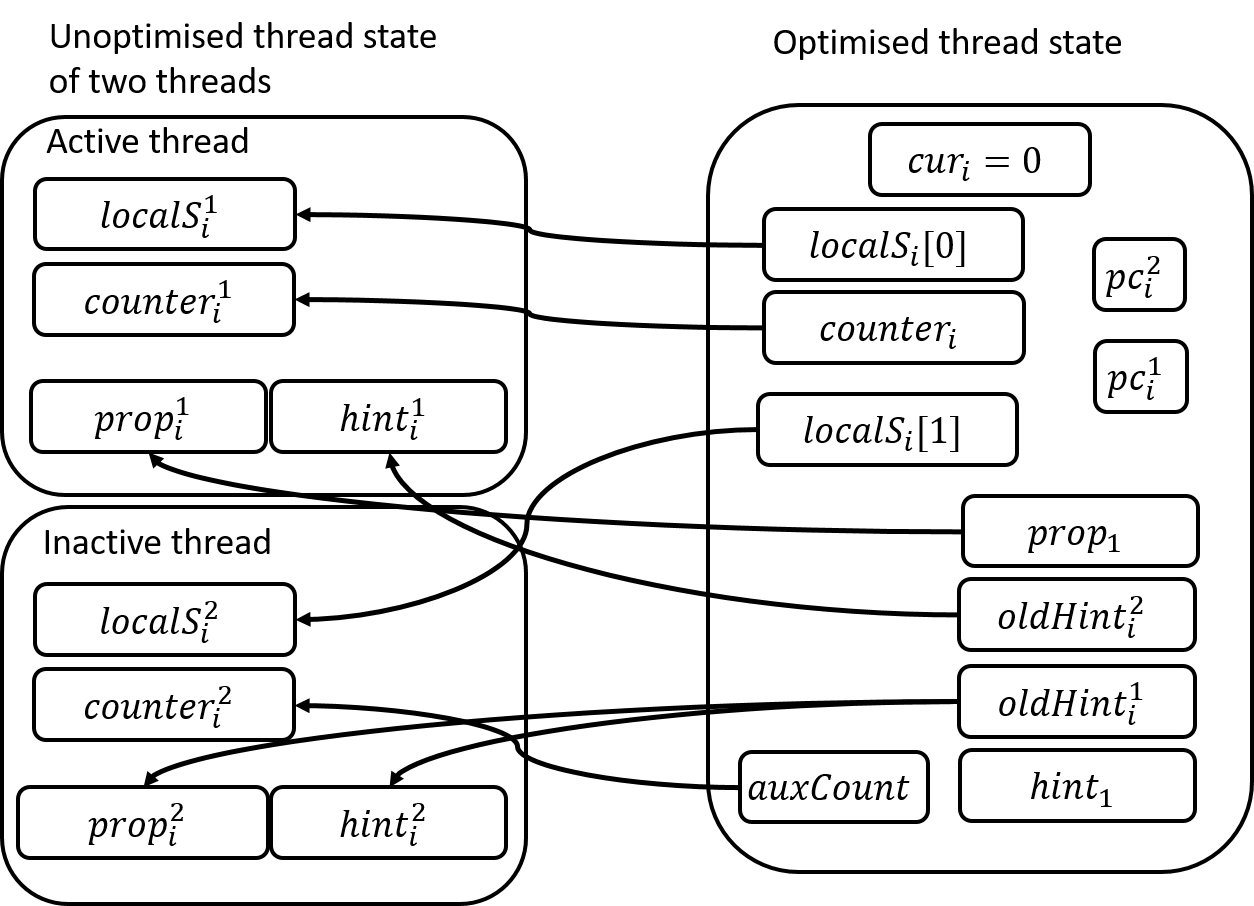
\includegraphics[width=5in]{images/optConcurrentMap.png}
    \caption{Reference mapping of $g$ when $cur_i$ equals 0 before executing lines 127.}
    \label{fig:optConcurrentMap}
\end{figure}

\begin{table}[H]
    \begin{tabular}{c|c|c}
        \emph{OptParSketch} line & \emph{ParSketch} line & Executing thread\\[5pt]
        \hline
        \ref{l:checkfull} & \ref{l:checkfull} & $t_i^0$\\[5pt]
        \ref{l:wait} & \ref{l:wait}& $t_i^1$\\[5pt]
        \ref{opt:l:swap-local-aux} & - & - \\[5pt]
        \ref{l:updateHint} & \ref{l:updateHint} & $t_i^1$\\[5pt]
        \ref{l:zeroCounter} & \ref{l:zeroCounter} & $t_i^1$\\[5pt]
        \ref{opt:l:signal} & \ref{l:signal} & $t_i^0$ 
    \end{tabular}
    \caption{Example for steps taken by $t_i^0$ and $t_i^1$ for each step taken by $t_i$ when $cur_i=0$ before line~\ref{l:checkfull},
    meaning the ``round'' of $b$ updates was ingested by $t_i^0$. On line~\ref{opt:l:swap-local-aux} neither thread takes a step.}
    \label{table:opt-simulation}
\end{table}

We also define the steps taken in $ParSketch$ when $OptParSketch$ takes a step. If a \emph{query} is invoked,
then both algorithms take the same step. If an \emph{update} in invoked, the an \emph{update} is invoked in
$t[cur_i]$ in $ParSketch$. If the counter gets up to $b$ (meaning we get to line~\ref{l:wait}), then
$t[1-cur_i]$ executes line~\ref{l:wait}. When $OptParSketch$ flips $cur_i$ (line~\ref{opt:l:swap-local-aux}),
then neither threads $t_i^0$ or $t_i^1$ take a step. Afterwards, lines \ref{l:updateHint} and \ref{l:zeroCounter}
execute the respective lines on thread $t[cur_i]$, and line \ref{opt:l:signal} executes \ref{l:signal} on thread $t[1-cur_i]$.

\begin{lemma}
    $g$ is a simulation relation from $OptParSketch$ to $ParSketch$.
\end{lemma}
\begin{proof}
The proof is by induction on the steps in an execution. In the initial state, the mapping trivially holds.
In a given step, we refer to $t[{cur_i}]$ as the \emph{active} thread and $t[1-cur_i]$ as the \emph{inactive thread}. 
Query threads trivially map to themselves and do not alter the state. We next consider update and propagator threads. 
Consider first the steps of OptParSketch that execute the corresponding step on the active thread.
These are lines 119-123 and 127-128.
All of these steps have a direct one-to-one correspondence with the same steps of ParSketch in the
active thread ($t[cur_i]$), and except in line 127 abd 129, the effected state variables are mapped to the
same state variables in the active thread. So these steps trivially preserve $g$.
Line 124 in \emph{ParSketch} is executed on the inactive thread when \emph{OptParSketch} executes line 129. As after
this step the inactive thread's prop and prop$_i$ are both 0, $g$ is preserved. 
Line 125 is executed on the inactive thread, waiting on the same variable, and modifies no variables, so $g$ is preserved.

Line 126 flips $cur_i$ and neither thread takes a step in \emph{ParSketch}. Here, the mappings of $prop$, $hint$, and $counter$ change. 
On this step oldHint$_i^1$ and oldHint$_i^2$ are updated as defined, and as $t_i$ is right before
executing line 127, oldHint$_i^1$ is equal to the inactive thread's ($t[1-cur_i]$) hint, and as before the step the (now)
inactive thread's prop was equal to hint$_i$, then after this step it is equal to oldHint$_i^0$.
As before the step the (now) active thread's hint was equal to oldHint$_i^1$, after this step it is equal to oldHint$_i^2$. Finally,
as before the step the (now) active thread's prop was equal to prop$_i$, after this step it remains equal to prop$_i$, so this
step preserve $g$.

In line 127, hint$_i$ gets the value of prop$_i$, and the same happens on the active thread. As before this line the
active thread's prop was equal to prop$_i$, after this step the inactive thread's prop and hint are equal to hint$_i$,
preserving $g$.
As the active thread's counter is equal to $counter_i$, line 128 preserves $g$.
The now inactive thread has filled its local sketch, therefore its counter is $b$, which equals
auxCount.  
Finally, the propagator thread’s steps (lines 110-115) execute on the inactive
thread and it is easy to see that all variables accessed in these steps are mapped to the same variables in the inactive thread. 
\end{proof}

Note that the simulation relation uses no prophecy variables, i.e., does not ``look into the future''.
Thus, the mapping of all ParSketch’s steps, including linearisation points,  to steps in OptParSketch is prefix-preserving.
Since we use two update threads of ParSketch to simulate one thread in OptParSketch, we have proven the following Theorem:
\optgenereicstrong*